% !TEX root = ./PS-Exercises_Resolutions.3.tex
\providecommand\mainfilename{"./PS-Exercises_Resolutions.tex"}
\providecommand \subfilename{}
\renewcommand   \subfilename{"./PS-Exercises_Resolutions.3.tex"}
\documentclass[\mainfilename]{subfiles}

% \tikzset{external/force remake=true} % - remake all

\begin{document}

\graphicspath{{\subfix{./figures/PS-Exercises_Resolutions.3}}}
\tikzsetexternalprefix{./figures/PS-Exercises_Resolutions.3/graphics/}

\mymakesubfile{3}
[PS]
{Resolução dos Exercicios: Extração Liq-Liq} % Subfile Title
{Resolução dos Exercicios: Extração Liq-Liq} % Part Title

\begin{questionBox}1{ % MARK: Q1
    Pretende-se extrair o ácido acético contido em \qty*{800}{\gram} de uma solução aquosa com 55\% (percentagem mássica de ácido acético) (\(T=\qty*{20}{\celsius}\)), adicionando-se \qty*{400}{\gram} de éter isopropílico, sem variação de temperatura.
} % Q1
    \paragraph*{Dados:}
    Para o sistema ternário éter isopropílico--água--ácido acético, as fases conjugadas têm a \qty*{20}{\celsius} as seguintes composições:
    \begin{center}
        \setlength\tabcolsep{1.5mm}        % width
        % \renewcommand\arraystretch{1.25} % height
        \vspace{1ex}
        \begin{tabular}{*{3}{C} | *{3}{C}}
            \toprule
            
                \multicolumn{3}{l}{Fase Orgânica}
                & \multicolumn{3}{l}{Fase Aquosa}
            
            \\\toprule

            \begin{tabular}{c}
                Éter\\isopropilico
            \end{tabular}
            & \begin{tabular}{c}
                Ácido\\Acético
            \end{tabular}
            & \multicolumn{1}{c|}{Água}
            & \begin{tabular}{c}
                Éter\\isopropilico
            \end{tabular}
            & \begin{tabular}{c}
                Ácido\\Acético
            \end{tabular}
            & \multicolumn{1}{c}{Água}

            \\\midrule
            
               98.80 & 0.00 & 1.20 & 0.80 & 0.00 & 99.20
            \\ 87.50 & 10.00 & 2.50 & 1.70 & 5.00 & 93.30
            \\ 76.20 & 20.00 & 3.80 & 2.10 & 10.00 & 87.90
            \\ 60.00 & 30.00 & 10.00 & 2.50 & 15.00 & 82.50
            \\ 39.00 & 41.50 & 19.50 & 3.30 & 25.00 & 71.70
            \\ 27.50 & 45.00 & 27.50 & 3.50 & 30.00 & 66.50
            \\ 19.70 & 46.80 & 33.50 & 4.20 & 35.00 & 60.80
            \\ 13.00 & 46.00 & 41.00 & 5.60 & 40.00 & 54.40
            
            \\\bottomrule
        \end{tabular}
        \vspace{2ex}

        
\includegraphics[width=.8\textwidth]{extractedPages-page5.pdf}
        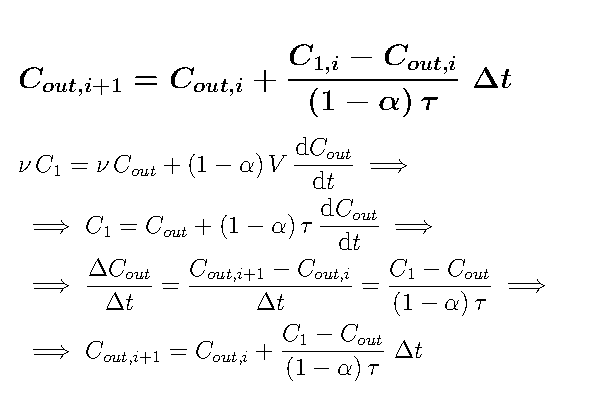
\includegraphics[width=.8\textwidth]{extractedPages-page6.pdf}
    \end{center}
\end{questionBox}

\begin{questionBox}2{ % MARK: Q1.1
    DeterDeterminar as composições e massas das fases em equilíbrio, depois da adição do éter
} % Q1.1
    \answer{}
    \begin{center}
        % \tikzset{external/remake next=true}
        \begin{tikzpicture}[xscale=3.5]
            \PSAndarScheme{1}
        \end{tikzpicture}
    \end{center}
    \begin{flalign*}
        &
            \text{Equilibrium}
            &\\&
            \begin{cases}
                \text{Feed}
                & x_F = 55\%
                \\ 
                \text{Solvent}
                & y_F = 0\%
            \end{cases}
            % 
            % 
            % 
            &\\[3ex]&
            \text{Finding midpoint M}
            &\\&
            x_{M,1}:
            m_F\,x_F+m_{S,1}\,y_{S,1}
            = m_{M,1}\,x_{M,1}
            = (m_F+m_{S,1})\,x_{M,1}
            \implies &\\&
            \implies
            x_{M,1}
            = \frac{m_F\,x_F+m_{S,1}\,y_{S,1}}{m_F+m_{S,1}}
            = \frac{800*.55+400*0}{800+400}
            \cong
            \qty{36.6666666666667}{\percent}
            \implies &\\&
            \implies
            M
            \begin{cases}
                x_{M.1,EAc}\cong& \qty[1]{36.666666666666667}{\percent}
                \\
                x_{M,1,Ether}\cong& 33\%
            \end{cases}
            % 
            % 
            % 
            ; &\\[3ex]&
            \text{Extract and Raffinate Points}
            &\\&
            E_1 \begin{cases}
                    y_{E,1,\ch{HAc}}& \cong 40.0\%
                \\  y_{E,1,\ch{Ether}}& \cong 41.5\%
            \end{cases}
            ; \qquad
            R_1 \begin{cases}
                    x_{R,1,\ch{HAc}}& \cong 22.0\%
                \\  x_{R,1,\ch{Ether}}& \cong  3.2\%
            \end{cases}
            % 
            % 
            % 
            ; &\\[3ex]&
            m_{E,1}\text{ e }m_{R,1}
            &\\&
            m_{E,1}:
            m_{E,1}\,y_{E,1}+m_{R,1}\,x_{R,1}
            = m_{E,1}\,y_{E,1}+(m_{M,1}-m_{E,1})\,x_{R,1}
            = &\\&
            = m_{M,1}\,x_{M,1}
            \implies &\\&
            \implies
            = m_{E,1}
            = m_{M,1}\,\frac{x_{M,1}-x_{R,1}}{y_{E,1}-x_{R,1}}
            \cong
            1200\,\frac
            {\num{0.36666666666666667}-0.220}
            {0.400-0.220}
            \cong
            \qty{902.564102564102769}{\gram}
            % 
            % 
            % 
            ; &\\[3ex]&
            m_{R_1}
            = m_M-m_{E_1}
            \cong 1200-\num{902.564102564102769}
            \cong \qty{297.435897435897231}{\gram}
        &
    \end{flalign*}
\end{questionBox}

\begin{sectionBox}*1{Mixing operation - Calculations} % MARK: S
    
    \paragraph*{Level--Arm Rule}
    \begin{BM}
        \begin{cases}
            \text{B.M. Global}& m_R+m_E=m_M
            \\
            \text{B.M. partial to C}& m_R\,x_R+m_E\,y_E=m_M\,x_M
        \end{cases}
        \implies
        \\
        \frac{m_R}{m_E}
        = \frac{\bar{M\,E}}{\bar{R\,M}}
        = \frac{x_M-y_E}{x_R-x_M}
        ; \qquad
        \frac{m_R}{m_M}
        = \frac{\bar{M\,E}}{\bar{R\,E}}
        = \frac{x_M-y_E}{x_R-x_E}
    \end{BM}
    
\end{sectionBox}

\begin{questionBox}2{ % MARK: Q1.2
    Para a remoção do ácido ainda existente na fase refinada obtida da operação anterior, adiciona-se éter isopropílico na proporção de 1:1. Determine as composições e as massas das novas fases em equilíbrio.
} % Q1.2
    \answer{}
    \begin{center}
        % \tikzset{external/remake next=true}
        \begin{tikzpicture}[xscale=3.5]
            \PSAndarScheme{2}
        \end{tikzpicture}
    \end{center}
    \begin{flalign*}
        &
            x_{M,2}:&\\&
            m_{M,2}\,x_{M,2}
            = (m_{R,1}+m_{S,2})\,x_{M,2}
            = 2\,m_{R,1}\,x_{M,2}
            = &\\&
            = m_{R,1}\,x_{R,1}
            + m_{S,2}\,y_{S,2}
            = m_{R,1}\,(x_{R,1}+y_{S,2})
            \implies &\\&
            \implies
            x_{M,2}
            = \frac{x_{R,1}+y_{S,2}}{2}
            \cong \frac{22.0+0}{2}\%
            = 11.0\%
            % 
            % 
            % 
            % Traça o ponto no gráfico entre a reta R1xS2 e x=11.0%
            \implies &\\&
            \implies
            R_2\begin{cases}
                    \qty*{ 7}{\percent\of{HAc}}
                \\  \qty*{ 2}{\percent\of{Ether}}
                \\  \qty*{14}{\percent\of{Water}}
            \end{cases}
            ;\qquad
            E_2\begin{cases}
                    \qty*{14}{\percent\of{HAc}}
                \\  \qty*{83}{\percent\of{Ether}}
                \\  \qty*{ 3}{\percent\of{Water}}
            \end{cases}
            % 
            % 
            % 
            ; &\\[3ex]&
            m_{E,2}:&\\&
            m_{M,2}\,x_{M,2}
            = (M_{R,1}+m_{S,2})\,x_{M,2}
            = 2\,M_{R,1}\,x_{M,2}
            = &\\&
            = m_{E,2}\,y_{E,2}
            + m_{R,2}\,x_{R,2}
            = m_{E,2}\,y_{E,2}
            + (m_{M,2}-m_{E,2})\,x_{R,2}
            % 
            % 
            % 
            \implies &\\&
            \implies
            m_{E,2}
            = 2\,M_{R,1}\,\frac{x_{M,2}-x_{R,2}}{y_{E,2}-x_{R,2}}
            = 2*\num{297.435897435897231}
            \,\frac{11.0-7.0}{14.0-7.0}
            \cong &\\&
            \cong
            \qty{339.926739926739657}{\gram}
            % 
            % 
            % 
            \implies &\\[3ex]&
            \implies
            m_{R,2} &\\&
            m_{R,2}
            =m_{M,2}-m_{E,2}
            \cong
            2*\num{297.435897435897231}-\num{339.926739926739657}
            \cong 
            \qty{254.9450549450547}{\gram}
        &
    \end{flalign*}
\end{questionBox}

\begin{questionBox}1{ % MARK: Q2
    Pretende-se recuperar acetona de uma solução aquosa a \qty*{30}{\celsius} usando acetato de etilo, \ch{CH3COOCH2CH3}, como solvente. A corrente de alimentação, contendo 25\% de acetona e 75\% de água, entra no topo da coluna de extracção a um caudal de \qty*{250}{\kilo\gram/\hour}. O solvente, puro, entra na base a um caudal de \qty*{97}{\kilo\gram/\hour}. Deseja-se um produto refinado com 10\% de acetona. Calcule:
} % Q2
    \begin{center}
        \vspace{1ex}
        \begin{tabular}{*{3}{C}}
            \multicolumn{3}{l}{Dados de equilíbrio:}
            \\\toprule
            
                \begin{tabular}{c}
                    Acetato\\de etilo
                \end{tabular}
                & \multicolumn{1}{c}{Acetona}
                & \multicolumn{1}{c}{Água}
            
            \\\midrule
            
                7.4 & 0.0 & 92.6
            \\  8.0 & 7.6 & 84.4
            \\  9.9 & 16.1 & 74.0
            \\  11.9 & 21.1 & 67.0
            \\  13.6 & 24.3 & 62.1
            \\  15.5 & 27.0 & 57.5
            \\  17.4 & 29.2 & 53.4
            \\  19.2 & 31.1 & 49.7
            \\  24.0 & 33.8 & 42.2
            \\  25.5 & 34.6 & 39.9
            \\  29.0 & 36.0 & 35.0
            \\  36.7 & 37.0 & 26.3
            \\  44.4 & 36.1 & 19.5
            \\  47.6 & 35.0 & 17.4
            \\  55.0 & 32.0 & 13.0
            \\  62.5 & 27.5 & 10.0
            \\  70.0 & 22.4 & 7.6
            \\  77.0 & 17.0 & 6.0
            \\  83.7 & 11.2 & 5.1
            \\  96.5 & 0.0 & 3.5
            
            \\\bottomrule
        \end{tabular}

        \vspace{3ex}

        \setlength\tabcolsep{2mm}
        \begin{tabular}{*{3}{C} | *{3}{C}}
            \multicolumn{3}{l}{Fase organica:}
            & \multicolumn{3}{l}{Fase Aquosa:}

            \\\toprule
            
                \begin{tabular}{c}
                    Acetato\\de etilo
                \end{tabular}
                & \multicolumn{1}{c}{Acetona}
                & \multicolumn{1}{c|}{Água}
                & \begin{tabular}{c}
                    Acetato\\de etilo
                \end{tabular}
                & \multicolumn{1}{c}{Acetona}
                & \multicolumn{1}{c}{Água}
            
            \\\midrule
            
                91.0 & 4.8 & 4.2 & 8.3 & 3.2 & 88.5
            \\  85.6 & 9.4 & 5.0 & 8.0 & 6.0 & 86.0
            \\  80.5 & 13.5 & 6.0 & 8.3 & 9.5 & 82.2
            \\  77.2 & 16.6 & 6.2 & 9.2 & 12.8 & 78.0
            \\  73.0 & 20.0 & 7.0 & 9.8 & 14.8 & 75.4
            \\  70.0 & 22.4 & 7.6 & 10.2 & 17.5 & 72.3
            \\  65.0 & 26.0 & 9.0 & 12.2 & 19.8 & 68.0
            \\  62.0 & 27.8 & 10.2 & 11.8 & 21.2 & 67.0
            \\  54.0 & 32.6 & 13.4 & 15.0 & 26.4 & 58.6
            
            \\\bottomrule
        \end{tabular}
        \vspace{2ex}
    \end{center}
    \paragraph*{Acetato de etilo}
    \begin{itemize}
        \item Densidade (liq): \qty*{0.897}{\gram/\centi\metre^3}
        \item Ponto de Ebulição: \qty*{77}{\celsius}
    \end{itemize}
\end{questionBox}

\begin{questionBox}2{ % MARK: Q2.1
    A concentração e o caudal da corrente de extracto
} % Q2.1
    \answer{}
    \begin{flalign*}
        &
            \begin{cases}
                    AcEt:& \text{Acetato de Etilo}
                \\  Ac:& \text{Acetona}
                \\  \ch{H}:& \text{Agua}
            \end{cases}
            &\\&
            S:
            \begin{cases}
                y_S=0
                \\ \qty*{0}{\percent\of{Ac}}
                \\ \qty*{100}{\percent\of{AcEt}}
                \\ \qty*{0}{\percent\of{\ch{H2O}}}
            \end{cases}
            ; \qquad
            F:
            \begin{cases}
                y_F=0.75
                \\ \qty*{25}{\percent\of{Ac}}
                \\ \qty*{0}{\percent\of{AcEt}}
                \\ \qty*{75}{\percent\of{\ch{H2O}}}
            \end{cases}
            ; \qquad
            R_n:
            \begin{cases}
                y_{R,n}=0.75
                \\ \qty*{10}{\percent\of{Ac}}
                \\ \qty*{8.6}{\percent\of{AcEt}}
                \\ \qty*{81.4}{\percent\of{\ch{H2O}}}
            \end{cases}
            % 
            % 
            % 
            &\\[3ex]&
            x_{M,1}:
            &\\&
            m_{M,1}\,x_{M,1}
            = (m_{F}+m_{S,1})\,x_{M,1}
            = &\\&
            = m_{F}\,x_{F}
            + m_{S,1}\,y_{S,1}
            \implies &\\&
            \implies
            x_{M,1}
            = \frac{
                m_{F}\,x_{F}
                + m_{S,1}\,y_{S,1}
            }{
                m_{F}+m_{S,1}
            }
            = \frac{
                250*0.25
                + 97*0
            }{
                250+97
            }
            \cong &\\&
            \cong
            \qty{18.0115273775216}{\percent\of{Ac}}
            \implies &\\&
            \implies
            E_{1}:
            \begin{cases}
                y_{E,1}=0.30
                \\ \qty*{30}{\percent\of{Ac}}
                \\ \qty*{58.5}{\percent\of{AcEt}}
                \\ \qty*{11.5}{\percent\of{\ch{H2O}}}
            \end{cases}
            % 
            % 
            % 
            ; &\\[3ex]&
            m_{E,1}:
            &\\&
            m_{E,1}\,y_{E,1}
            + m_{R,n}\,x_{R,n}
            = m_{E,1}\,y_{E,1}
            + (m_{M,1}-m_{E,1})\,x_{R,n}
            = &\\&
            = m_{M,1}\,x_{M,1}
            \implies &\\&
            \implies
            m_{E,1}
            = m_{M,1}
            \,\frac
            {x_{M,1}-x_{R,n}}
            {y_{E,1}-x_{R,n}}
            \cong &\\&
            \cong 
            (250+97)
            \,\frac
            {\num{.180115273775216}-0.10}
            {0.30-0.10}
            \cong
            \qty{138.99999999999976}{\kilo\gram/\hour}
            \implies &\\&
            \implies
            m_{R,n}
            \cong 250+97-\num{138.99999999999976}
            \cong \qty{208.00000000000024}{\kilo\gram/\hour}
        &
    \end{flalign*}
\end{questionBox}

\begin{questionBox}2{ % MARK: Q2.2
    O número de andares de equilíbrio necessários para esta separação.
} % Q2.2
    \answer{}
    \begin{flalign*}
        &
            \Delta:
            &\\&
            F+S=E_1+R_{n,p}
            \implies &\\&
            \implies
            \Delta
            = F-E_1
            = R_{n,p}-S_1
            = R_i-E_{i+1}
            % Traçar no grafico 
            % - S->Rn->prolongando
            % - E_1->F->prolongando
            % - As retas devem se encontrar fora do gráfico, esse é o delta
            % 
            % 
            % 
            % Encontra y_{E,1} no segundo grafico na curva x=y
            % Traça horizontalmente até encontrar c a curva de eq
            % Esse é o ponto R_1
            % 
            % Traça: Delta->R_1->Curva do primeiro grafico
            % Esse ponto é o E_2
            % Repete até encontrar R_n (fica entre 2 valores)
        &
    \end{flalign*}
\end{questionBox}

\begin{sectionBox}*1b{Equilibrium Diagram for the system: Water, Kerosene, Nicotine} % MARK: S
    
    \begin{center}
        
\includegraphics[width=.8\textwidth]{extractedPages-page7.pdf}
    \end{center}
    
\end{sectionBox}

\begin{sectionBox}*1b{Equilibrium Diagram for the system: Water, Acetone, Ethyl acetate} % MARK: S
    
    \begin{center}
        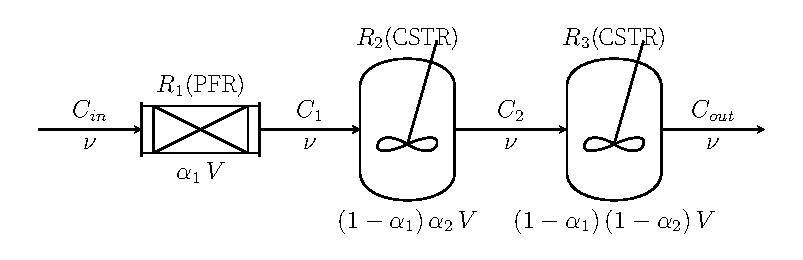
\includegraphics[width=.8\textwidth]{extractedPages-page8.pdf}
    \end{center}
    
\end{sectionBox}

\end{document}